\section{Theorie}
\label{sec:Theorie}

\subsection{Fehlerrechnung}

Für die Fehlerfortpflanzung bei Gleichungen mit $N$ fehlerbehafteten Größen
wird jeweils die Formel zur Gaußschen Fehlerfortpflanzung

\begin{equation}
  \sigma = \sqrt{\sum_{i=1}^{N}\biggl(\frac{\partial f(x_i)}{\partial x_i}
  \sigma_i\biggr)^2}
\end{equation}
mit der jeweiligen Funktion $f(x_i)$, den Messgrößen $x_i$ und den
zugehörigen Fehlern $\sigma_i$ verwendet.
Zur Berechnung des arithmetischen Mittels von $N$ Messwerten wird jeweils die
Formel

\begin{equation}
  \bar{x} = \frac{1}{N}\sum_{i=1}^{N}x_i
\end{equation}
mit den Messwerten $x_i$ benutzt.
Die Standardabweichung des Mittelwerts wird jeweils mit der Gleichung

\begin{equation}
  \bar{\sigma} = \sqrt{\frac{1}{N-1}\sum_{i=1}^{N}(x_i - \bar{x})^2}
\end{equation}
mit den $N$ Messwerten $x_i$ berechnet.

\subsection{Einleitung und Zielsetzung}

In der Kernphysik wird das Geiger-Müller-Zählrohr zur Messung
radioaktiver Strahlung benutzt. Das Messinstrument ist in der Lage, elektrische
Impulse bei Strahlungseinfall zu erzeugen, die dann mit Hilfe eines
Impulszählers gemessen werden können.
Im folgenden Versuch sollen die wichtigsten Kenndaten eines
Geiger-Müller-Zählrohrs bestimmt werden.

\subsection{Aufbau und Wirkungsweise}

In Abbildung \ref{fig:GMZ} ist eine Skizze für das Zählrohr abgebildet.
In dem Kathoden-Zylinder aus Stahl mit dem Radius $r_k$ befindet sich zentral
ein Anoden-Draht mit dem Radius $r_a$ und ein Gasgemisch, vorzugsweise Argon
und Ethylalkohol.
Um das Ansprechvermögen für eintreffende, radioaktive Strahlung zu vergrößern,
ist das Eintrittsfenster aus Mylar, einer sehr dünnen Folie. Diese ist
aufgrund des Unterdrucks nach innen gewölbt.
Wird eine äußere Spannung zwischen Kathode und Anode angelegt, so entsteht
im Zylinder ein radialsymmetrisches, elektrisches Feld mit der Feldstärke
\begin{align}
  E(r) = \frac{U}{r\ln(r_k/r_a)}.
\end{align}

\begin{figure}
  \centering
  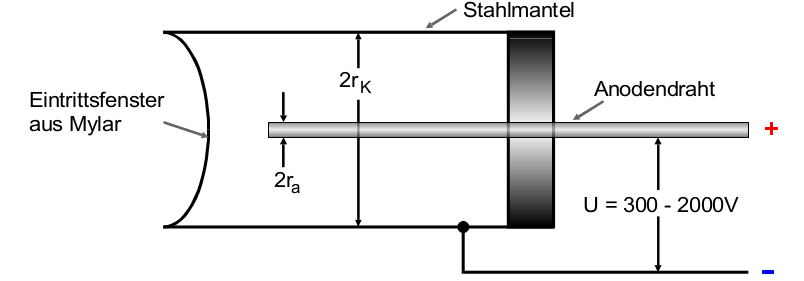
\includegraphics[height=3.8cm]{MeinePics;)/GMZ.png}
  \caption{.\cite{anleitung}}
  \label{fig:GMZ}
\end{figure}

\FloatBarrier

Energiereiche Teilchen, die durch das Eintrittsfenster in den Zylinder
gelangen,
bewegen sich durch das Gasgemisch und ionisieren die Argon-Atome,
bis ihre Energie aufgebraucht ist. Die entstehenden
Elektronen bewegen sich zum Anodendraht und können dort detektiert werden.
Die Menge an detektierten Ladungen hängt von der Spannung ab.
In Abbildung \ref{fig:EU} ist diese Abhängigkeit skizziert.
Im ersten Bereich, bei sehr geringer Spannung, rekombinieren die Ionenpaare
unmittelbar nach ihrer Enstehung, da sie nicht genügend beschleunigt werden.
Die Rekombinationswahrscheinlichkeit sinkt mit steigender Spannung schnell ab,
sodass im zweiten Spannungs-Bereich bereits alle erzeugten Elektronen zum
Anodendraht gelangen. In diesem Bereich sind die detektierten Ladungen
proportional zur einfallenden Strahlung, sodass $\alpha$- und $\beta$-Strahlung
aufgrund ihrer verschiedenen Energien unterschieden werden können.
Die sogenannte Ionisationskammer, die unter derartigen Spannungen
arbeitet, wird allerdings nur bei hohen Strahlungsintensitäten benutzt.
Im nächsten Spannungsbereich werden die entstehenden Elektronen so beschleunigt,
dass sie ein anderes Atom ionisieren. Dieses Phänomen wird als
Stoßionisation bezeichnet.
Durch lawinenartige Zunahme der freien Elektronen kann die an der Anode
gesammelte Ladung bereits als Ladungsimpuls gemessen werden. Da die
Ladung $Q$ proportional zur Energie des eintreffenden Teilchens ist, können
in diesem Spannungsbereich sowohl Aussagen über Strahlungsintensität, als auch
Strahlungsenergie gemacht werden. Ein Detektor, der mit dieser Spannung
arbeitet, wird daher auch als Proportionalzählrohr bezeichnet.
Der vierte Spannungsbereich ist der Auslöse- oder auch Geiger-Müller-Bereich.
Bei der Anregung der Argonatome durch die Elektronenlawine entstehen bei dieser
Spannung UV-Photonen, welche sich im Gegensatz zu den Elektronen in alle
Richtungen ausbreiten können, da sie ladungsneutral sind. Die Elektronenlawinen
werden so im ganzen Zählrohr ausgelöst und hängen nur noch von Spannung und
Volumen und nicht mehr von der Strahlungsenergie ab. Bei dieser Spannung
kann also nur die Strahlungsintensität gemessen werden, jedoch mit sehr
geringem elektronischem Aufwand, da die detektierten Ladungen sehr groß sind.

\begin{figure}
  \centering
  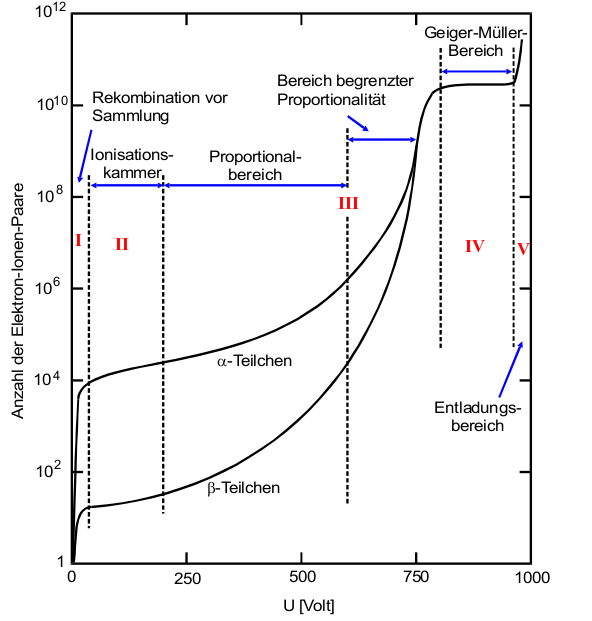
\includegraphics[height=10cm]{MeinePics;)/EU.png}
  \caption{.\cite{anleitung}}
  \label{fig:EU}
\end{figure}

\FloatBarrier

\subsection{Totzeit und Nachentladungen}

Als Totzeit $T$ bezeichnet man die Zeitspanne, in der kaum Stoßionisationen im
Zählrohr stattfinden, da dort eine positive, radialsymmetrische Raumladung
aufgebaut wurde. Diese entsteht, da sich die positiven Ionen,
die aus der Ionisation enstehen, nur, verglichen den Elektronen, langsam
zur Kathode bewegen und das elektrische Feld daher abschwächen.
Mit der Zeit bewegt sich die positive Ladungswolke zur Kathode und
es können wieder Teilchen detektiert werden.
Die ursprüngliche Ladung $Q$ wird allerdings erst wieder gemessen, wenn alle
Kationen wieder neutralisiert wurden. Als Erholungszeit $T_E$ wird die
Zeitspanne vom Ende der Totzeit bis zur vollständigen Neutralisierung
bezeichnet.
In Abbildung \ref{fig:TOT} ist die Tot- und Erholungszeitspanne skizziert.

\begin{figure}
  \centering
  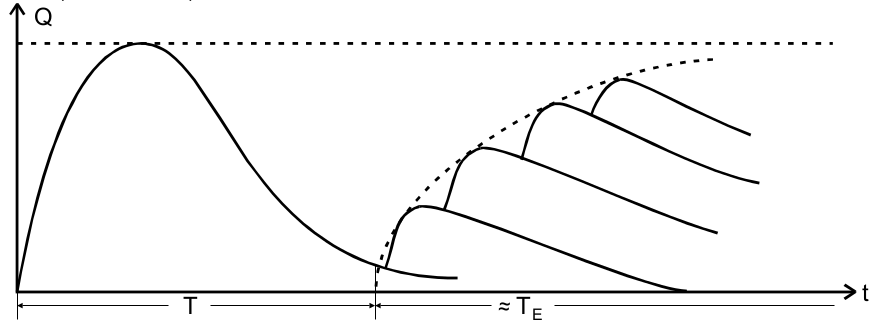
\includegraphics[height=4cm]{MeinePics;)/TOT.png}
  \caption{.\cite{anleitung}}
  \label{fig:TOT}
\end{figure}

Die zur Kathode wandernden Ionen können aus dem Zählrohrmantel Elektronen lösen,
die dann durch das E-Feld zur Anode beschleunigt werden. Diese sogenannten
Sekundärelektronen können wiederum eine Lawine auslösen, sodass weitere
elektrische Impulse detektiert werden, obwohl kein neues hochenergetisches
Teilchen in das Zählrohr gelangt ist. Dieses unerwünschte Phänomen
wird als Nachentladung bezeichnet. Um dies zu verhindern, wird
Ethylalkohol als Zusatz zum Gasgemisch hinzugefügt. Die Edelgasionen, die
sich zur Kathode bewegen, stoßen mit den Alkoholmolekülen zusammen und
ionisieren diese. Die Alkoholionen bewegen sich erneut nach außen, aufgrund
ihrer negativen Ladung, lösen aber keine Elektronen aus dem Mantel, da
die freiwerdende Energie zu niedrig ist. Dadurch entstehen keine Nachentladung
und es werden nur einfliegende Teilchen vom Zählrohr detektiert.

\subsection{Charakteristik des Zählrohrs}

In Abbildung \ref{fig:GMB} ist die sogenannte Charakteristik des
Geiger-Müller-Zählrohrs, also die registrierte Teilchenzahl $N$ gegen die
Spannung $U$ bei konstanter Strahlungsintensität, skizziert.

\begin{figure}
  \centering
  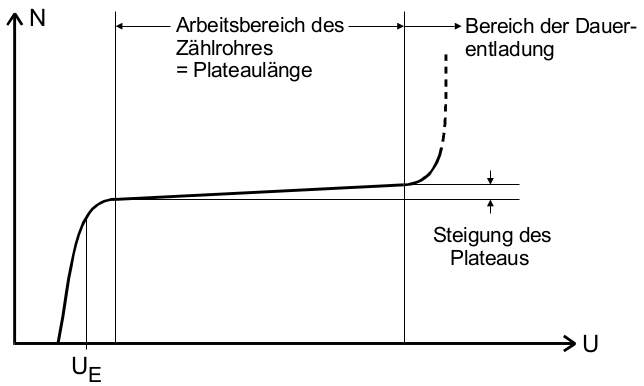
\includegraphics[height=5cm]{MeinePics;)/GMB.png}
  \caption{.\cite{anleitung}}
  \label{fig:GMB}
\end{figure}

\FloatBarrier

Der lineare Teil der Kurve, der etwa bei der Auslösespannung $U_E$ beginnt,
wird als Plateau bezeichnet.
Beim idealen Zählrohr ist die Steigung dieser Geraden Null. Da aber mit
steigender Spannung immer einige wenige Nachentladungen detektiert werden,
hat die Gerade beim realen Zählrohr eine Steigung $m > 0$.
In dem Bereich der Dauerentladung hinter der Gerade steigt die Zahl der
Nachentladungen drastisch und somit auch die detektierten Impulse.
Bei dieser Spannung endlädt sich das Gas selbstständig.

\subsection{Zwei-Quellen-Methode}

Mit Hilfe der Zwei-Quellen-Methode kann die Totzeit eines Zählrohrs bestimmt
werden.
Für die "wahre" Impulsrate, also die Menge an eintreffenden Teilchen pro
Zeit, gilt
\begin{align}
  N_\text{w} = \frac{\text{Impulsrate}}{\text{Messzeit}} =
  \frac{N_\text{r}}{1-TN_\text{r}}
  \label{eqn:WahreRate}
\end{align}
mit der Totzeit $T$ und der gemessenen Impulsrate $N_\text{r}$.
Mit zwei radioaktiven Materialien werden die Zählraten
$N_1, N_{1+2}$ und $N_2$ bei jeweils gleichen Bedingungen gemessen.
Für die wahren Impulsraten gilt
\begin{align}
  N_\text{{w,}1+2} = N_\text{w,1} + N_\text{w,2},
  \label{eqn:WahreAdd}
\end{align}
da aber mit Totzeit gemessen wird ist
\begin{align}
  N_{1+2} < N_1 + N_2.
\end{align}
Aus Gleichung \eqref{eqn:WahreRate} folgen die Beziehungen zwischen
$N_\text{w,1}$ und $N_1$, $N_\text{w,2}$ und $N_2$ und
$N_{\text{w,}1+2}$ und $N_{1+2}$
und mit \eqref{eqn:WahreAdd} ergibt sich
\begin{align}
  \frac{N_{1+2}}{1-TN_{1+2}} = \frac{N_1}{1-TN_1} + \frac{N_2}{1-TN_2}
  \label{eqn:tot1}
\end{align}
Aus \eqref{eqn:tot1} folgt die Totzeit $T$ in Abhängigkeit von den Messwerten
\begin{align}
  T = \frac{1}{N_{1+2}} - \sqrt{\frac{1}{N_{1+2}^2}-\frac{N_1 + N_2 - N_{1+2}}{N_1 N_2 N_{1+2}}}.
\end{align}

\subsection{Zählrohr-Ladungsmenge pro Teilchen}

Für den mittleren Zählrohrstrom gilt
\begin{align}
  & \bar{I} = \frac{1}{\tau} \int_{0}^{\tau} \frac{U(t)}{R} \symup{d}t & & \tau >> T.
\end{align}
Daraus ergibt sich für die pro Zeiteinheit $\increment t$ transportierte Ladung
\begin{align}
  \increment Q = \bar{I} \frac{\increment t}{Z}
\end{align}
mit der registrierten Teilchzahl $Z$.
